\chapter{Evaluation}

\section{Introduction}

In this chapter, we investigate the performance characteristics of the two runtimes we created for FrDataFlow. We will explore different types of reactive programs and how they behave under high loads of data, comparing them on a few metrics. More specifically, we will focus on the following metrics:

\begin{description}[style=nextline]
  \item [Latency]		The time it takes for a value to propagate through the entire graph of signals
  \item [Throughput]	The amount of values that can propagate through the entire graph within a certain time frame.
  \item [Scaling]		The amount of performance that can be gained by executing the program in parallel
\end{description}

These objective measurements can provide us with meaningful insight as to how efficient both interpreters are, and what the effects of parallelization are for our benchmarks.

\newpage
\section{Topologies}

Before we can start running benchmarks, we must first define the types of programs that we are interested in profiling. In \textit{Optimizing Distributed REScala} \cite{drechsler_optimizing_2014}, three topologies are suggested that sufficiently represent any reactive program for the purposes of evaluating performance.

\subsection{Linear}

This model is the simplest one: we have a graph of signals where each signal only has one parent and one child. When the source signal emits a new value, it simply propagates through the graph in one linear motion and stops at the end. 

\begin{figure}[h]
	\centerline{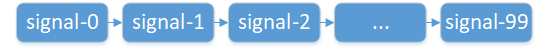
\includegraphics[scale=0.7]{images/Evaluation-Topologies-Linear.png}}
	\caption{A linear topology: each signal has one parent and one child}
	\label{fig:evaluation-topologies-linear}
\end{figure}

\subsection{Fan out}

In this topology, our graph immediately splits up into many children, as shown in figure \ref{fig:evaluation-topologies-fanout}. This is a scenario where one source signal provides important data that every other signal depends upon. The interesting effect of this is when that specific source signal emits a new value, it will trigger an immediate high load of updates for all of its children. 

\begin{figure}[h]
	\centerline{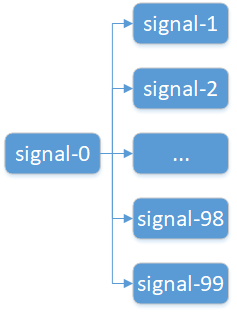
\includegraphics[scale=0.7]{images/Evaluation-Topologies-Fanout.png}}
	\caption{A fan-out topology: one signal with a large amount of children}
	\label{fig:evaluation-topologies-fanout}
\end{figure}

\subsection{Square}

The square topology is expected to be the most common, it provides a signal graph that is not extremely deep such as the linear topology nor is it very wide like the fan-out variant. In this topology, signals have a variable amount of parents and children, shaping the graph into a square. For the purposes of our benchmarks, we will use an exact square graph for simplicity.  

\begin{figure}[h]
	\centerline{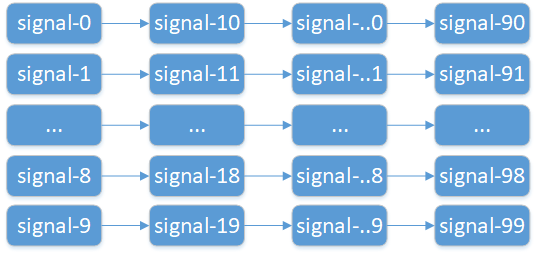
\includegraphics[scale=0.7]{images/Evaluation-Topologies-Square.png}}
	\caption{A square topology: The signal graph is equally deep as it is wide}
	\label{fig:evaluation-topologies-square}
\end{figure}

\section{Benchmarks}

All of the benchmarks in this chapter are run in the Racket VM with unlimited memory (16 GB RAM physical limit) and on an AMD Phenom II X4 955 processor (Quad core, 3.2 GHz). Three sample programs were created with around 100 signals each, each of which implementing one of the three topologies as shown in the diagrams. These programs were each executed three times for 60 seconds, taking the averages of the output to produce the charts in this chapter.
A single source signal was emulated to emit 10 million values per second and the output nodes of the signal graphs were inspected to collect information on how many values were propagate through the graph and at what rate the update mechanisms could keep up with the stream of incoming data. 

\newpage
\subsection{Without dataflow engine}

We will first evaluate the runtime that implements an update loop in the interpreter itself and does not use the dataflow model to keep its graphs up to date. These are the tests for our first runtime for FrDataFlow. 

\subsubsection{Latency}

\begin{figure}[h]
	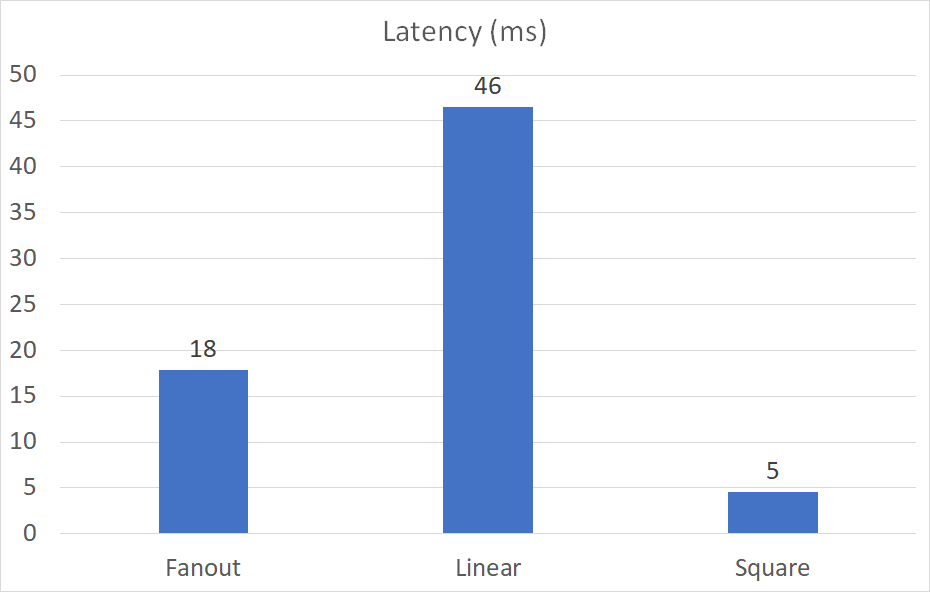
\includegraphics[width=\textwidth]{images/Evaluation-WithoutDataFlow-Latency.png}
	\caption{The latency of signals in FrDataFlow without the dataflow engine}
	\label{fig:evaluation-withoutdataflow-latency}
\end{figure}

Inspecting these results, we conclude that the linear graph show the highest latency, which is expectable: values in this topology travel the longest path of signals before they reach the end. On average, it took nearly 50 ms for a value to propagate from the source signal to the last output node.
More interestingly, values in the fanout topology seem to take longer on average to reach the end than in the square variant. This is counterintuitive, because every value in the fanout graph only needs to pass two signal nodes before it reaches the end. Since the fanout graph contains 99 output nodes and the square graph only 10, it would seem that this gives the square graph a slight edge: these 10 output nodes have to wait less long to be given the chance to announce their output. 

\subsubsection{Throughput}

\begin{figure}[h]
	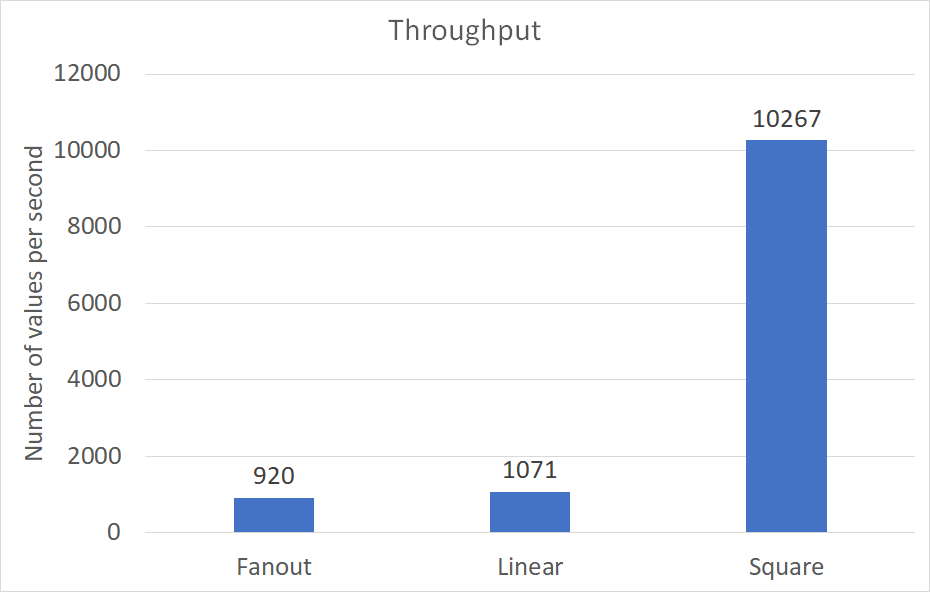
\includegraphics[width=\textwidth]{images/Evaluation-WithoutDataFlow-Throughput.png}
	\caption{The throughput of signals in FrDataFlow without the dataflow engine}
	\label{fig:evaluation-withoutdataflow-throughput}
\end{figure}

Even more so than with latency, the square topology is the clear winner when it comes to the sheer amount of values it can push through the graph per second. The square graph can push out more than 10 000 values per second and is an order of magnitude more efficient compared to the fanout or linear approach, who only managed to process 1 000 values by and large. This makes sense, because every update loop iterates over all the signal nodes once. In the square topology, this means it can propagate 10 values to the end in one loop. The linear version on the other hand can only process one, because when the iteration is happening it is really pushing forward one value from the first signal all the way to the last. Similarly, the fanout approach results in one loop pushing a single value from the first signal to all other signals. The square topology, by splitting up the graph in 10 linear parts, essentially 
parallelizes this work. 

\section{With dataflow engine}

In this section, we repeat the same tests of the previous section but this time using the runtime that sits atop the dataflow engine. The programs are exactly the same, but they are now compiled to dataflow instructions and invoked there. These are the tests for our second runtime for FrDataFlow. 

\subsection{Latency}

\begin{figure}[h]
    \includegraphics[width=\textwidth]{images/Evaluation-WithDataFlow-Latency.png}
	\caption{The latency of signals in FrDataFlow with the dataflow engine}
	\label{fig:evaluation-withdataflow-latency}
\end{figure}

The first thing that is immediately obvious is the increase in latency. While the relative proportions remain the same (the square topology is slightly better than fanout, while the linear topology is clearly the worst in this regard) we observe an average of 50 ms extra latency because we now translate to dataflow instructions. This was to be expected: the use of a dataflow engine brings with it some extra overhead such as the management of the token queue. While 50 ms is considerable, it is not a show stopping performance penalty and is thus acceptable for the gains that can be made in other spaces.

\subsection{Throughput}

\begin{figure}[h]
	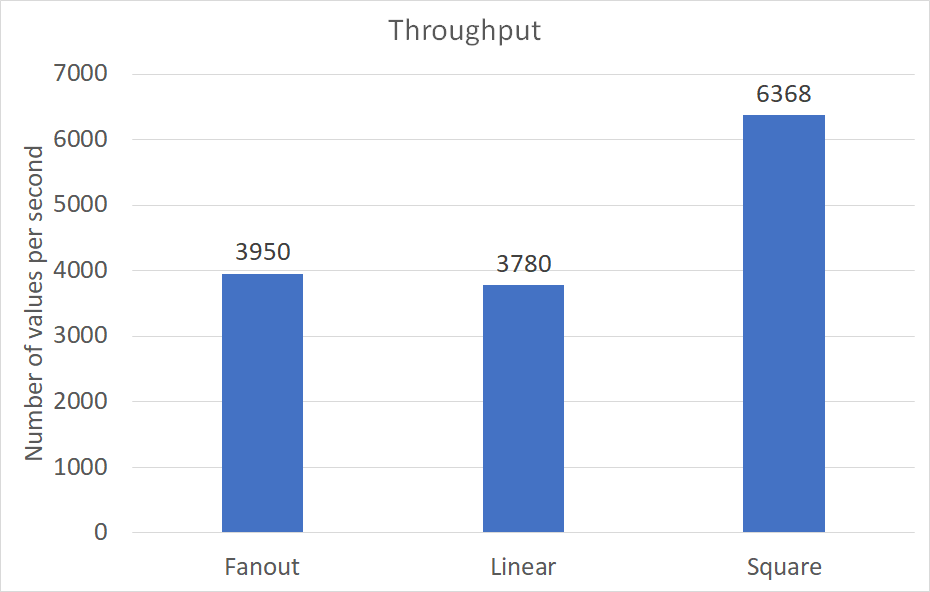
\includegraphics[width=\textwidth]{images/Evaluation-WithDataFlow-Throughput.png}
	\caption{The throughput of signals in FrDataFlow with the dataflow engine}
	\label{fig:evaluation-withdataflow-throughput}
\end{figure}

\subsection{Without parallelization}

\subsection{With parallelization}

\section{Conclusion}
